\documentclass[12pt,a4pape, fullpage]{article}
\usepackage[
margin=1.5cm,
includefoot,
footskip=30pt,
]{geometry}
\usepackage[utf8]{inputenc}
%\usepackage[T1]{fontenc}
\usepackage{amsmath}
\usepackage{amsfonts}
\usepackage{amssymb}
\usepackage{graphicx}
\usepackage{comment}
\usepackage{natbib}
\usepackage{lineno}

\bibliographystyle{evolution.bst}

\newcommand{\norm}[1]{\left\lVert#1\right\rVert}
\newcommand{\normsq}[1]{\left\lVert#1\right\rVert^2}


\newcommand{\MX}{\mathbf{X}} %uncentered data
\newcommand{\MC}{\mathbf{C}} %centering
\newcommand{\MY}{\mathbf{Y}} %centered data
\newcommand{\MF}{\mathbf{F}_2} %F2-distance matrix
\newcommand{\MFT}{\mathbf{F}_3} %F3-distance matrix
\newcommand{\MP}{\mathbf{P}} % PCs
\newcommand{\ML}{\mathbf{L}} % loadings
\newcommand{\MK}{\mathbf{K}} % Kernel
\newcommand{\MSINGULAR}{\mathbf{\Sigma}} % Singular values matrix
\newcommand{\MEIGEN}{\mathbf{\Lambda}} % Eigenvalue matrix


\newcommand{\MEAN}{\boldsymbol{\mu}} % Kernel
\begin{document}
\section{Introduction}
About 15\% of genetic variation in humans can be explained by population structure \cite{lewontin1972, barbujani1997, rosenberg2003}, but the information contained in these 15\% is sufficient to study the genetic diversity and history in great detail \cite{edwards2003}. For some data sets it is possible to predict an individuals origin at a resolution of a few hundred kilometers \cite{novembre2008, leslie2015}, and direct-to-consumer-genetics companies are using this variation to analyze the genetic data of millions of customers.

In Lewontin's pioneering analysis, he found that less than half (6\%), of that variation could be attributed to the continental-scale groups he called races, it seemed  which he used to claim that ''racial classification is (...) seen to be of virtually no genetic or taxonomic significance``.

One related question is how discrete human populations are. While human genetic differentiation generally increases with geographic distance \cite{ramachandran2005, rosenberg2007}, this increase is not uniform. Obstacles to migration,  such as oceans, mountains or deserts do frequently cause discontinuities in population structure \cite{peter2020a}. Thus, while barriers to gene flow rarely are absolute, segregation policies by (perceived) ethnic or racial ancestry frequently cause local small-scale population differentiation that persist to the present day.

Thus, it frequently a useful analysis tool to think of populations as discrete units. For example, even though the underlying population structure may be continuous, sampling is not; and when quantifying ascertainment and sampling biases, or when discussing population structure it is often helpful to pretend populations are discrete, even though the underlying structure is typically more complex. This leads to challenges both in data interpretation and communication, and often researchers will analyze a data set both using methods that assume population structure is discrete, and methods where this assumption does not need to be made.

One discrete framework for the analysis of human population structure that gained a lot of traction in the last decade are the $F$-statistics \textit{sensu} Patterson \cite{patterson2012, peter2016}. This framework treats populations as discrete units in the analysis, and allows for a variety of tests for treeness. Using this framwork, the vast majority of present-day human populations are admixed \cite{pickrell2014}. Yet, this framework starts with the assumption that admixture is i) rare and ii) discrete.

However, $F$-statistics are not restricted to discrete populations. Indeed, as they can be written as functions of allele frequency variances, or expected pairwise coalescence times, statistics that can be calculated under a wide range of demographic models \cite{peter2016}. Indeed, as they reflect inner products, they can be generalized to Euclidean space \cite{oteo2021} (or any Hilbert space, although we won't pursue that here).
Here, I explore these links between $F$-statistics and Euclidean spaces to establish connections between $F$-statistics and PCA. This allows direct interpretation of admixture in scenarios where population structure might not be discrete.




Particularly for the analysis of ancient DNA, two approaches have been proven to be particularly useful: one are global summary analyses, such as Structure \citep{pritchard2000, alexander2009} Principal Component Analysis (PCA) \citep{cavalli-sforza1994, reich2008, novembre2008, mcvean2009} and classical multidimensional scaling (MDS) \cite{fu2016, malaspinas_bammds}. Typically, these methods assume that population structure is \emph{sparse}, so that a low-rank approximation with few underlying ``components'' is sufficient to model population structure See e.g. \cite{engelhardt2010} for a useful perspective how these approaches are related.

Facing a novel data set, PCA or MDS are often the first analyses (beyond quality controls) a researcher performs, in order to obtain insights in the general population structure they are faced with. In order to answer more specific questions and to test specific hypotheses, the $F$-statistic framework of \cite{patterson2012} has been proven particularly powerful (see also \cite{peter2016} for a more gentle introduction). In the $F$-statistic framework, usually only a small number of populations are used at once, to e.g. test for treeness and find closely related populations.

Even though these two approaches are considered in almost every ancient DNA paper, links between the inferences made from them are usually only compared qualitatively. In this paper, our goal is to show that PCA and $F$-statistics are in fact closely related by construction, and use a very similar summary of the data. 


\subsection{Introduction to $F$-statistics}
$F$-statistics have been primarily motivated by trees and admixture graphs \citep{patterson2012, peter2016}, but the calculations hold up in a much wider data space. In particular,  \cite{oteo-garcia2021} provides a thorough introduction to interpreting $F$-statistics in the \emph{data space} $\mathbb{R}^k$. Their work builds much of the foundation of this discussion, by demonstrating analogies to classical geometry. A brief summary of their key results: A population's allele frequencies can be thought of as vector in $\mathbb{R}^k$. Then, $F_2(X_1, X_2) = \normsq{X_1 - X_2}$ is the squared Euclidean distance between the populations with vectors $X_1$ and $X_2$, and $F_4(X_1, X_2 ; X_3, X_4) = \langle X_1 - X_2, X_3 - X_4 \rangle$ is the inner (scalar) product between these two vectors. Here, I will mainly use the $F$-statistic notation, but use the geometric notation where convenient.



	
\section{Relationship of PCA, $F_2$ and Outgroup-$F_3$}

The goal of this section is to give a cursory introduction to $F$-statistics, PCA and MDS, and to define notation. A more detailed technical introduction is given in XXXXX, and a useful guide to interpretation is \cite{cavalli-sforza1994}.

\subsection{Introduction to PCA}
	Let us assume we have some genotype data summarized in a matrix $\MX$, where the entry $x_{ij}$ is the allele frequency of the $i$-th population at the $j$-th genotype. If we have $k$ SNPs and $n$ populations, $\MX$ will have dimension $n \times k$. 
	
    As a population may be represented by just one (pseudo-)haploid or diploid individual, there is no conceptual difference between these cases and I will refer to populations as unit for analysis, for simplicity. 
    
    Since the allele frequencies are between zero and one, we can interpret each row $x_i$ of $\MX$ as a vector in $[0, 1]^k$, the \emph{data space} of all possible allele frequencies on our markers.
	
	The goal of a PCA is to find a low-dimensional representation of this data space that retains most of the data (see Fig. \ref{fig:pca_explanation} for an intuitive explanation). 
	
	\begin{figure}
		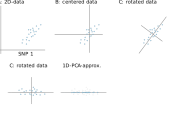
\includegraphics[width=\textwidth]{pca_explanation.png}
		\caption{Basic Idea of PCA from 2D to 1D representation. A: Allele frequencies from different populations (blue dots) at two SNPs. A PCA is performed by centering the data (B), and rotating it (B) such that the first PC explains the majority of variation in the data, and the second PC is orthognal to the first, and explains the residual. A lower-dimensional approximation (in this case 1D) can be achieved by just keeping the first PC (E); which can be translated back to the original data space by inverting the rotation and centering (F).}
		\label{fig:pca_explanation}
	\end{figure}
	
	There are several algorithms that are used to calculate a PCA in practice, the most common one relies on a singular value decomposition. In this approach, we first mean-center $\MX$, obtaining a centered matrix $\MY$
	\begin{equation}
	y_{il} = x_{il} - \mu_l
	\end{equation}
	where $\mu_l$ is the mean allele frequency at the $l$-th locus.
	
	PCA can then be written as
	
	\begin{equation}
	\MY = \MC\MX = \mathbf{U} \MSINGULAR \mathbf{V}^T = \MP\ML\text{,}
	\end{equation}
	
	where $\MC = \mathbf{I} -\frac{1}{n}\mathbf{1}$ is a centering matrix that subtracts row means, with $\mathbf{I}, \mathbf{1}$  the identity matrix and a matrix of ones, respectively. The orthogonal matrix of principal components $\MP=\mathbf{U}\MSINGULAR$ has size $n \times n$ and is used to reveal population structure. The loadings $\ML=\mathbf{V}^T$ are an orthonormal matrix of size $n \times k$, its rows give the contribution of each SNP to each PC, it is often useful to look for outliers that might be indicative of selection \cite[e.g][]{francois2010}.
	
	In many  implementations \citep[e.g]{patterson2006}, SNPs are weighted by the inverse of their standard deviation. As this weighting makes little difference in practice, I will for now assume that SNPs are unweighted, and defer discussion of weighting to a later section.
	
	Equivalently, we obtain the PCs by performing an eigendecomposition of the  covariance matrix denoted as $\MK$:
	 \begin{equation}
 \MK = \MY \MY^T = \mathbf{U}\MEIGEN\mathbf{U}^T = \mathbf{U}\MSINGULAR^2\mathbf{U}^T =\MP\MP^T
	\end{equation} where $\MEIGEN$ is the diagonal matrix with the eigenvalues of $\MK$. 
	This algorithm does not compute the SNP-loadings. However, the $i$-th row of $L$  can be obtained from $\MP$ and the original data, whenever the eigenvalue $\lambda_i \neq 0$:
	\begin{equation}
	\ML_i = \lambda_i^{-1}\MP^T\MC\MX \text{.}
	\end{equation}
	



\section{$F$-statistics in PCA-space}
As shown by e.g. \cite{oteo-garcia2021}, $F$-statistics can be thought of as inner products in Euclidean space, and $F_2$ is an (estimated) squared Euclidean distance between two populations in allele frequency space. By performing a PCA, we just translate and rotate our data, but Euclidean distances and dot products are both invariant under both these operations. Hence, neither mean-centering (a translation) nor PCA (a rotation) will change $F_2$. What this means is that we are free to calculate $F_2$ either on the uncentered data $\MX$, the centered data $\MY$ or the principal components $\MP$. Formally,

\begin{align}
F_2(X_i, X_j) &=&  \sum_{l=1}^L \big( x_{il} -x_{jl}\big)^2 - H_i - H_j &&\nonumber\\ 
 &=& \sum_{l=1}^L \big( (x_{il} - \mu_l) -(x_{jl} -\mu_l)\big)^2 - H_i - H_j  &=& F_2(Y_i, Y_j) \nonumber\\
 &=& \sum_k (P_{ik} - P_{jk})^2 - H_i - H_j &=& F_2(P_i, P_j) \text{,}
\end{align}
where $H_i$ and $H_j$ are the bias-correction terms proposed in \cite{reich2009}. A detailed derivation of this is given in Appendix \ref{appendix:fonpc}.
As $F_3$ and $F_4$ can be written as sums of $F_2$-terms, analogous relations apply.

\subsection{$F$-stats in 2-dimensional PC-space}
The transformation derived in the previous section allows us to consider the geometry of $F$-statistics in PCA-space. The relationships we will discuss formally only hold if we use all $n-1$ PCs. However, the appeal of PCA is that frequently, only a very small number $K \ll n$ of PCS contain most information that is relevant for population structure.

Here, we start by discussing 2-dimensional spaces. This is useful for two reasons: for one, the geometry is simpler and we can think of circles and squares as opposed to $n$-balls and other high-dimensional geometric objects and thus build intuition. Second, in many applications it is argued that a 2-dimensional approximation is sufficient to explain the major components of population structure \cite{novembre2008}. In this case, the results here will hold under the same approximation assumptions in low-dimensional PCs; if they differ substantially from each other, it is likely that not sufficiently many PCs were considered.


\subsubsection{$F_2$ in PC-space}
The $F_2$-statistic is an estimate of the squared Euclidean distance is the easiest to understand, it corresponds directly to the squared distance in PCA-space. This matches our intuition that closely related populations (which have low $F_2$) will be close to each other on a PCA-plot.




\subsubsection{$F_3$ and circles}
The $F_3$-statistic becomes more interesting; as outlines above we either think of $F_3$ as ``outgroup''-$F$-stats or as admixture $F$-stats. In the admixture case, we may ask the following question: given two source populations $X_1$, $X_2$, where would admixed populations on a PCA plot lie? From theory, we would expect it to lie between $X_1$ and $X_2$, with the exact location depending on sample sizes \cite{brisbin2012, mcvean2009}. 

Formally, we would reject admixture if $F_3$ is negative, i.e. we are looking for the space
\begin{eqnarray}
2 F_3(X_x; X_1, X_2) &=& 2\langle  X_x - X_1, X_x - X_2 \rangle \nonumber\\
      &=& \normsq{X_x - X_1} + \normsq{X_x - X_2}  - \normsq{X_1 - X_2} \nonumber\\
      &<&0
\end{eqnarray}
By the Pythagorean theorem, $F_3 = 0 $ iff $X_1, X_2$ and $X_x$ form a right-angled triangle. Hence, the region where $F_3$ is zero is the circle with diameter through $X_1$ and $X_2$. If $X_x$ lies inside this circle, the angle is obtuse and $F_3$ is negative, otherwise it will be positive. Similarly, if we fix $X_1$ and $X_2$ and ask where on a 2D-PCA-plot $X_2$ would lie, this space is defined by all the points for which the angle between $X_1 X_x$ and $X_2 X_x$ is obtuse.

This highlights a potential identifiability issue with $F_3$: Since all values of $F_3$ that result in the same projection will give the same value; and multiple admixture events may result in the same $F_3$-value.

\begin{figure}[!ht]
	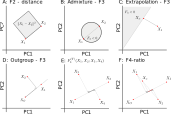
\includegraphics[width=\textwidth]{dummy_pca.png}
	\caption{\textbf{Geometric representation of $F$-statistics on 2D-PCA-plot.} A: $F_2$ represents the squared Euclidean distance between two points in PC-space. B: Admixture-$F_3(X_x; X_1, X_2)$ is negative if $X_x$ lies in the circle specified by the diameter $X_2-X_1$}. C: $F_3(X_x; X_1, X_2)$ is negative given $X_1, X_x$ if $X_2$ is in the gray space.  D: Outgroup-$F_3$ reflects the projection of $X_2 - X_O$ on $X_1 - X_O$. E: $F_4$ is the projection of $X_3 - X_4$ on $X_1-X_2$. F: If $X_x$ is admixed between $X_1$ and $X_2$, the admixture proportions will be projected.
\end{figure}

\subsubsection{$F_4$ and right angles}
The inner-product-interpretation of $F_4$ is similar to that of $F_3$, with the change that the two vectors we consider do not involve the same population. However, a finding of $F_4(X_1, X_2; X_3, X_4) = \langle X_1 - X_2, X_3 - X4 \rangle = 0$ similarly implies that the two vectors are orthogonal, and a non-zero value reflects the projection of one vector on the other.

\subsubsection{$F_4$-ratio}
\begin{eqnarray}
\frac{F_4(X_I, X_O; X_X, X_1)}{F_4(X_I, X_O; X_2, X_1)} &=& \frac{\norm{X_I-X_O}\norm{X_X-X_1}\cos(\alpha)}{\norm{X_I-X_O}\norm{X_2-X_1}\cos(\beta)}\nonumber\\
&=&\frac{\norm{X_X-X_1}\cos(\alpha)}{\norm{X_2-X_1}\cos(\beta)}\nonumber\\
&=& \frac{\norm{X_X' - X_1'}}{\norm{X_2' - X_1'}}
\end{eqnarray}
where $\alpha$ and $\beta$ are the angles between vectors, and $X_i'$ is the projection of $X_i$ on $X_I-X_O$.

Conjecture: Thus, we are measuring the distances between the admixing populations on the projected on the axis between $X_I$ and $X_O$. This ought to be valid only if $\langle X_1 - X_1', X_2 - X_2' \rangle$ are orthogonal to each other, and to $X_OX_I$, i.e.
$F_4(X_1, X_1', X_2, X_2') = 0$
 
	
\subsection{Higher-Dimensional Spaces}


\section{Trees and admixture graphs in PCA-space}
\subsection{Trees}
Evolutionary trees are fundamental in phylogenetic analyses, as they, on a large, scale, approximate how taxa diversify. Within a species, applying trees is also very common, but more problematic as populations frequently do not evolve as discrete lineages; instead, they admix and diversify as much more continuous processes. This is largely due to the time-scales involved, speciation events that give rise to trees might often be similarly messy, but from a distance of millions of years these issues might disappear. 

Thus, when estimating trees from population genetic data, we must be very careful about whether the data is actually consistent with a tree, or belongs to some wider class of model.


Trees can be thought of as a collection of orthogonal dimensions; as drift on each branch is independent from every other branch. Thus, each sample is only 
\begin{enumerate}
	\item Trees
	\item Admixture Graphs
	\item Treelets
	\item simple trees, admixture graph
\end{enumerate}


\section{Technical considerations}
	\subsection{SNP weighting}
	It is clear that weighting SNP will have some effect on the resulting PCAs. Upweighting rare variants e.g. will emphasis recent events, as rare variance in the sample are more likely to be recent.
	
	
	\subsection{Missing data}
	
	\subsection{$F_2$ error}
	In most $F$-statistics applications, $F_2$ is \emph{estimated} using the minimum-variance unbiased estimator \citep{reich2009}
	\begin{subequations}

	\begin{equation}
	f_2(X_1, X_2) = \frac{1}{L}\sum_l (x_{l1} - x_{l2})^2 - \frac{1}{L}\sum_l\frac{x_{l1} (1-x_{l1})}{n_{l1}-1} - 
	\frac{1}{L}\sum_l\frac{x_{l2} (1-x_{l2})}{n_{l2}-1} - 
	\end{equation}
	in contrast, as shown above, PCA can be thought as a decomposition of a matrix of uncorrected $F_2$-statistics:
	\begin{equation}
	F_2(X_1, X_2) = \frac{1}{L}\sum_l(x_{l1} - x_{l2})^2
	\end{equation}
	\end{subequations}

	This leads to some issues, for example trying to perform a PCA on the matrix of $f_2$-values is not positive semidefinite, and so some principal components may be imaginary. One possible resolution is probabilistic PCA \citep[e.g.][]{engelhardt2010,agrawal2020}.
	
	\begin{align}
	    y_{ij} | \MP_{ij}, \epsilon_i &= (\MP\ML)_{ij} + \epsilon_{ij}\nonumber\\
	    x_i & \sim N(0, \mathbf{I}) \nonumber\\
	    \epsilon_i &\sim N(0, \sigma^2 \mathbf{I})\nonumber
	\end{align}
	
	\subsection{qpADM}
	In \cite{haak2015}, qpADM, a procedure to estimate admixture proportions has been proposed. qpADM aims to solve equations of the form
	
	\begin{align}
	\langle P_X - A, B -C \rangle &= \sum_i  \alpha_i\langle R_i - A, B - C \rangle \nonumber\\
	&= \left\langle \sum_i  \alpha_i R_i - A, B - C \right\rangle
	\end{align}
	
	
	\subsection{What is a dimension?}
	In both the PCA and $F$-statistic framework, a population at  a particular point in time can be thought of as a single point in allele-frequency space, given by the $k$-dimensional vector $v_0$ of allele frequencies at the $k$ SNPs in that population. If this population evolves for some time in isolation, allele frequencies will change due to genetic drift from $v_0$ to some other point $v_1$. Likewise, a second population with frequency $w_0$ will move to $w_1$. Crucially, if these populations do not interact, the changes in allele frequency, $v_1 - v_0$ and $w_1 - w_0$ will be uncorrelated \cite{patterson2012}. Thus, if we have two populations that descend from the same ancestral population in isolation, they can be thought of as evolving along orthognal dimensions from the same point. This argument is at the foundation of F-statistics.
	
	
	\section{outtakes}
	PCA from $\MX$
	\begin{equation}
	\MK = \MY \MY^T = \MC\MX\MX^T \MC = \MP\MP^T
	\end{equation}

\section{Discussion}
The fa



\appendix
\section{Derivation}\label{appendix:fonpc}
\begin{eqnarray}
F_2(X_i, X_j) &=& \sum_{l=1}^L \big( (x_{il} - \mu_l) -(x_{jl} -\mu_l)\big)^2 = F_2(Y_i, Y_j)\nonumber\\
&=& \sum_{l=1}^L \big( \sum_k L_{kl}P_{ik} - \sum_kL_{kl}P_{kj}\big)^2\nonumber\\
&=& \sum_{l=1}^L \left( \sum_k L_{kl} (P_{ik} -P_{jk}) \right)^2\nonumber\\
&=& \sum_{l=1}^L \left( \sum_k L_{kl}^2 (P_{ik} -P_{jk})^2 + 2\sum_{k\neq k'} L_{kl}L_{k'l}(P_{ik} - P_{jk'})^2 \right)\nonumber\\
&=& \sum_k \underbrace{\left(\sum_{l=1}^L L_{kl}^2\right)}_1 (P_{ik} -P_{jk})^2 + \sum_{k\neq k'}\underbrace{\left(\sum_{l=1}^L L_{kl}L_{k'l}\right)}_{0} (P_{ik} - P_{jk'})^2\nonumber\\
&=& \sum_k (P_{ik} - P_{jk})^2
\end{eqnarray}

In summary, the first row shows that $F_2$ on the centered data will give the same results (as distances are invariant to translations), in the second row we apply the PC-decomposition. The third row is obtained from factoring out $L_{lk}$. Row four is obtained by multiplying out the sum inside the square term for a particular $l$. We have $k$ terms when for $\binom{k}{2}$ terms for different $k$'s.  Row five is obtained by expanding the outer sum and grouping terms by $k$.The final line is obtained by recognizing that $\ML$ is an orthonormal basis; where dot products of different vectors have lengths zero.

Note that if we estimate $F_2$, unbiased estimators are obtained by subtracting the population-heterozygosities $H_i, H_j$ from the statistic. As these are scalars, they do not change above calculation.
\bibliography{main}

\end{document}
